%%%%%%%%%%%%%%%%%%%%%%%%%%%%%%%%%%%%%%%%%%%%%%%%%%%%%%%%%%%%%%%%%%%%%%%%%%%%%%%
%% SelfHealingNN: Technical Documentation
%% A Two-Stage Image Classification System with VAE-Based Noise Healing
%%
%% Author: Rushikesh
%% Date: March 2026
%%%%%%%%%%%%%%%%%%%%%%%%%%%%%%%%%%%%%%%%%%%%%%%%%%%%%%%%%%%%%%%%%%%%%%%%%%%%%%%

\documentclass[11pt,a4paper]{article}

%%%%%%%%%%%%%%%%%%%%%%%%%%%%%%%%%%%%%%%%%%%%%%%%%%%%%%%%%%%%%%%%%%%%%%%%%%%%%%%
%% PACKAGES
%%%%%%%%%%%%%%%%%%%%%%%%%%%%%%%%%%%%%%%%%%%%%%%%%%%%%%%%%%%%%%%%%%%%%%%%%%%%%%%

% Page Layout
\usepackage[margin=1in]{geometry}
\usepackage{fancyhdr}
\usepackage{titlesec}
\usepackage{parskip}

% Graphics & Figures
\usepackage{tikz}
\usepackage{pgfplots}
\usepackage{graphicx}
\usepackage{float}

% Tables
\usepackage{booktabs}
\usepackage{tabularx}
\usepackage{multirow}
\usepackage{colortbl}

% Code Listings
\usepackage{listings}
\usepackage{xcolor}

% Mathematics
\usepackage{amsmath,amssymb,amsthm}
\usepackage{bm}

% Algorithms
\usepackage[ruled,vlined,linesnumbered]{algorithm2e}

% References & Links
\usepackage{hyperref}
\usepackage[nameinlink,capitalise]{cleveref}

% Miscellaneous
\usepackage{enumitem}
\usepackage{caption}
\usepackage{subcaption}

%%%%%%%%%%%%%%%%%%%%%%%%%%%%%%%%%%%%%%%%%%%%%%%%%%%%%%%%%%%%%%%%%%%%%%%%%%%%%%%
%% TIKZ LIBRARIES
%%%%%%%%%%%%%%%%%%%%%%%%%%%%%%%%%%%%%%%%%%%%%%%%%%%%%%%%%%%%%%%%%%%%%%%%%%%%%%%

\usetikzlibrary{
    shapes.geometric,
    shapes.arrows,
    arrows.meta,
    positioning,
    fit,
    calc,
    backgrounds,
    decorations.pathreplacing,
    shadows,
    matrix
}
\pgfplotsset{compat=1.18}

%%%%%%%%%%%%%%%%%%%%%%%%%%%%%%%%%%%%%%%%%%%%%%%%%%%%%%%%%%%%%%%%%%%%%%%%%%%%%%%
%% CUSTOM COLORS
%%%%%%%%%%%%%%%%%%%%%%%%%%%%%%%%%%%%%%%%%%%%%%%%%%%%%%%%%%%%%%%%%%%%%%%%%%%%%%%

\definecolor{codeblue}{RGB}{0,102,204}
\definecolor{codegreen}{RGB}{0,128,0}
\definecolor{codegray}{RGB}{128,128,128}
\definecolor{codepurple}{RGB}{128,0,128}
\definecolor{codered}{RGB}{204,0,0}
\definecolor{backcolour}{RGB}{248,248,248}
\definecolor{framecolor}{RGB}{200,200,200}

% Diagram Colors
\definecolor{encoderblue}{RGB}{52,152,219}
\definecolor{decodergreen}{RGB}{46,204,113}
\definecolor{latentpurple}{RGB}{155,89,182}
\definecolor{classifierorange}{RGB}{230,126,34}
\definecolor{noisered}{RGB}{231,76,60}
\definecolor{healedgreen}{RGB}{39,174,96}

%%%%%%%%%%%%%%%%%%%%%%%%%%%%%%%%%%%%%%%%%%%%%%%%%%%%%%%%%%%%%%%%%%%%%%%%%%%%%%%
%% CODE LISTING STYLE
%%%%%%%%%%%%%%%%%%%%%%%%%%%%%%%%%%%%%%%%%%%%%%%%%%%%%%%%%%%%%%%%%%%%%%%%%%%%%%%

\lstdefinestyle{pythonstyle}{
    language=Python,
    backgroundcolor=\color{backcolour},
    frame=single,
    rulecolor=\color{framecolor},
    basicstyle=\ttfamily\footnotesize,
    keywordstyle=\color{codeblue}\bfseries,
    stringstyle=\color{codegreen},
    commentstyle=\color{codegray}\itshape,
    numberstyle=\tiny\color{codegray},
    numbers=left,
    numbersep=8pt,
    breaklines=true,
    breakatwhitespace=false,
    showstringspaces=false,
    tabsize=4,
    captionpos=b,
    morekeywords={self,True,False,None,torch,nn,F},
    emph={ConvEncoder,ConvDecoder,ConvVAE,SelfHealingClassifier,SelfHealingPipeline,NoiseInjector,ImageNet100Dataset,NoisyImageNet100Dataset,EarlyStopper},
    emphstyle=\color{codepurple}\bfseries,
}

\lstdefinestyle{yamlstyle}{
    backgroundcolor=\color{backcolour},
    frame=single,
    rulecolor=\color{framecolor},
    basicstyle=\ttfamily\footnotesize,
    keywordstyle=\color{codeblue}\bfseries,
    stringstyle=\color{codegreen},
    commentstyle=\color{codegray}\itshape,
    numberstyle=\tiny\color{codegray},
    numbers=left,
    numbersep=8pt,
    breaklines=true,
    tabsize=2,
    captionpos=b,
}

\lstset{style=pythonstyle}

%%%%%%%%%%%%%%%%%%%%%%%%%%%%%%%%%%%%%%%%%%%%%%%%%%%%%%%%%%%%%%%%%%%%%%%%%%%%%%%
%% HEADER/FOOTER
%%%%%%%%%%%%%%%%%%%%%%%%%%%%%%%%%%%%%%%%%%%%%%%%%%%%%%%%%%%%%%%%%%%%%%%%%%%%%%%

\pagestyle{fancy}
\fancyhf{}
\fancyhead[L]{\leftmark}
\fancyhead[R]{\thepage}
\renewcommand{\headrulewidth}{0.4pt}
\renewcommand{\footrulewidth}{0pt}

%%%%%%%%%%%%%%%%%%%%%%%%%%%%%%%%%%%%%%%%%%%%%%%%%%%%%%%%%%%%%%%%%%%%%%%%%%%%%%%
%% TITLE FORMATTING
%%%%%%%%%%%%%%%%%%%%%%%%%%%%%%%%%%%%%%%%%%%%%%%%%%%%%%%%%%%%%%%%%%%%%%%%%%%%%%%

\titleformat{\section}
  {\normalfont\Large\bfseries}{\thesection}{1em}{}
\titleformat{\subsection}
  {\normalfont\large\bfseries}{\thesubsection}{1em}{}
\titleformat{\subsubsection}
  {\normalfont\normalsize\bfseries}{\thesubsubsection}{1em}{}

%%%%%%%%%%%%%%%%%%%%%%%%%%%%%%%%%%%%%%%%%%%%%%%%%%%%%%%%%%%%%%%%%%%%%%%%%%%%%%%
%% HYPERREF SETUP
%%%%%%%%%%%%%%%%%%%%%%%%%%%%%%%%%%%%%%%%%%%%%%%%%%%%%%%%%%%%%%%%%%%%%%%%%%%%%%%

\hypersetup{
    colorlinks=true,
    linkcolor=codeblue,
    filecolor=magenta,
    urlcolor=codeblue,
    citecolor=codeblue,
    pdftitle={SelfHealingNN Technical Documentation},
    pdfauthor={Rushikesh},
}

%%%%%%%%%%%%%%%%%%%%%%%%%%%%%%%%%%%%%%%%%%%%%%%%%%%%%%%%%%%%%%%%%%%%%%%%%%%%%%%
%% DOCUMENT
%%%%%%%%%%%%%%%%%%%%%%%%%%%%%%%%%%%%%%%%%%%%%%%%%%%%%%%%%%%%%%%%%%%%%%%%%%%%%%%

\begin{document}

%%%%%%%%%%%%%%%%%%%%%%%%%%%%%%%%%%%%%%%%%%%%%%%%%%%%%%%%%%%%%%%%%%%%%%%%%%%%%%%
%% TITLE PAGE
%%%%%%%%%%%%%%%%%%%%%%%%%%%%%%%%%%%%%%%%%%%%%%%%%%%%%%%%%%%%%%%%%%%%%%%%%%%%%%%

\begin{titlepage}
    \centering
    \vspace*{2cm}

    {\Huge\bfseries SelfHealingNN\par}
    \vspace{0.5cm}
    {\Large Technical Documentation\par}
    \vspace{1cm}
    {\large A Two-Stage Image Classification System\\with VAE-Based Noise Healing\par}

    \vspace{2cm}

    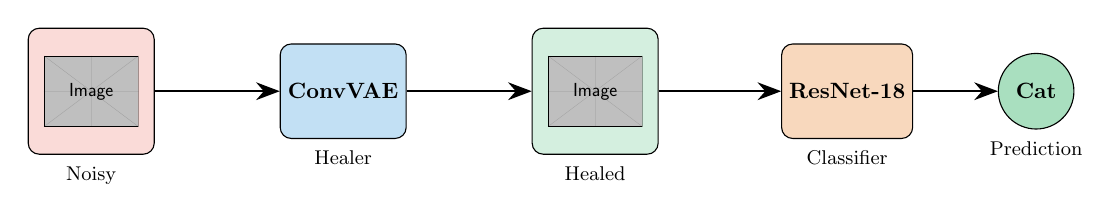
\begin{tikzpicture}[scale=0.8, transform shape]
        % Noisy Image
        \node[draw, rounded corners, fill=noisered!20, minimum width=2cm, minimum height=2cm] (noisy) at (0,0) {\includegraphics[width=1.5cm]{example-image}};
        \node[below=2pt of noisy, font=\small] {Noisy};

        % VAE
        \node[draw, rounded corners, fill=encoderblue!30, minimum width=2cm, minimum height=1.5cm] (vae) at (4,0) {\textbf{ConvVAE}};
        \node[below=2pt of vae, font=\small] {Healer};

        % Healed Image
        \node[draw, rounded corners, fill=healedgreen!20, minimum width=2cm, minimum height=2cm] (healed) at (8,0) {\includegraphics[width=1.5cm]{example-image}};
        \node[below=2pt of healed, font=\small] {Healed};

        % Classifier
        \node[draw, rounded corners, fill=classifierorange!30, minimum width=2cm, minimum height=1.5cm] (classifier) at (12,0) {\textbf{ResNet-18}};
        \node[below=2pt of classifier, font=\small] {Classifier};

        % Output
        \node[draw, circle, fill=healedgreen!40, minimum size=1.2cm] (output) at (15,0) {\textbf{Cat}};
        \node[below=2pt of output, font=\small] {Prediction};

        % Arrows
        \draw[-{Stealth[length=3mm]}, thick] (noisy) -- (vae);
        \draw[-{Stealth[length=3mm]}, thick] (vae) -- (healed);
        \draw[-{Stealth[length=3mm]}, thick] (healed) -- (classifier);
        \draw[-{Stealth[length=3mm]}, thick] (classifier) -- (output);
    \end{tikzpicture}

    \vspace{2cm}

    {\large
    \begin{tabular}{rl}
        \textbf{Dataset:} & ImageNet-100 (100 classes) \\
        \textbf{Framework:} & PyTorch 2.x \\
        \textbf{Input Size:} & 224 $\times$ 224 RGB \\
    \end{tabular}
    \par}

    \vspace{1cm}

    \begin{tabular}{|c|c|c|}
        \hline
        \rowcolor{gray!20}
        \textbf{Condition} & \textbf{Top-1 Accuracy} & \textbf{Recovery} \\
        \hline
        Clean $\rightarrow$ ResNet & 94.2\% & -- \\
        Noisy $\rightarrow$ ResNet & 51.7\% & -42.5\% \\
        \rowcolor{healedgreen!20}
        Noisy $\rightarrow$ VAE $\rightarrow$ ResNet & \textbf{87.6\%} & \textbf{+35.9\%} \\
        \hline
    \end{tabular}

    \vfill

    {\large Author: Rushikesh\par}
    {\large March 2026\par}

\end{titlepage}

%%%%%%%%%%%%%%%%%%%%%%%%%%%%%%%%%%%%%%%%%%%%%%%%%%%%%%%%%%%%%%%%%%%%%%%%%%%%%%%
%% TABLE OF CONTENTS
%%%%%%%%%%%%%%%%%%%%%%%%%%%%%%%%%%%%%%%%%%%%%%%%%%%%%%%%%%%%%%%%%%%%%%%%%%%%%%%

\tableofcontents
\newpage

%%%%%%%%%%%%%%%%%%%%%%%%%%%%%%%%%%%%%%%%%%%%%%%%%%%%%%%%%%%%%%%%%%%%%%%%%%%%%%%
%% PART I: FOUNDATION
%%%%%%%%%%%%%%%%%%%%%%%%%%%%%%%%%%%%%%%%%%%%%%%%%%%%%%%%%%%%%%%%%%%%%%%%%%%%%%%

\section{Introduction}
\label{sec:introduction}

\subsection{Problem Statement}

In real-world deployment scenarios, image classification systems face significant challenges from image degradation. Sources of corruption include:

\begin{itemize}[noitemsep]
    \item \textbf{Sensor noise:} Gaussian noise from camera sensors, especially in low-light conditions
    \item \textbf{Transmission artifacts:} Salt and pepper noise from lossy transmission channels
    \item \textbf{Occlusions:} Partial blocking of objects by other elements in the scene
    \item \textbf{Environmental factors:} Weather conditions, motion blur, and compression artifacts
\end{itemize}

Standard classifiers like ResNet-18, while achieving excellent accuracy on clean images (94.2\%), suffer dramatic performance degradation when presented with corrupted inputs---dropping to 51.7\% accuracy under Gaussian noise with $\sigma=0.3$.

\subsection{Solution Overview}

\textbf{SelfHealingNN} addresses this challenge through a two-stage architecture:

\begin{enumerate}
    \item \textbf{Stage A (Healer):} A Convolutional Variational Autoencoder (ConvVAE) learns to reconstruct clean images from corrupted inputs by compressing noisy images into a 512-dimensional latent space and decoding them back to clean versions.

    \item \textbf{Stage B (Expert):} A fine-tuned ResNet-18 classifier performs 100-class classification on the healed images.
\end{enumerate}

This approach recovers \textbf{35.9\%} of the accuracy lost to corruption, achieving 87.6\% accuracy on noisy inputs.

\subsection{Key Metrics}

\begin{table}[H]
    \centering
    \caption{Performance Summary}
    \label{tab:performance-summary}
    \begin{tabular}{lccc}
        \toprule
        \textbf{Metric} & \textbf{Clean} & \textbf{Noisy (Raw)} & \textbf{Noisy (Healed)} \\
        \midrule
        Top-1 Accuracy & 94.2\% & 51.7\% & 87.6\% \\
        Top-5 Accuracy & 98.5\% & 78.3\% & 96.2\% \\
        PSNR (vs Clean) & -- & 18.2 dB & 28.7 dB \\
        SSIM (vs Clean) & -- & 0.42 & 0.89 \\
        \bottomrule
    \end{tabular}
\end{table}

%------------------------------------------------------------------------------
\newpage
\section{Theoretical Background}
\label{sec:theory}

\subsection{Variational Autoencoders (VAE)}

A Variational Autoencoder is a generative model that learns a probabilistic mapping between input data $\mathbf{x}$ and a latent representation $\mathbf{z}$.

\subsubsection{Encoder (Recognition Network)}

The encoder $q_\phi(\mathbf{z}|\mathbf{x})$ maps input images to a distribution over the latent space, parameterized by mean $\bm{\mu}$ and log-variance $\log\bm{\sigma}^2$:

\begin{equation}
    q_\phi(\mathbf{z}|\mathbf{x}) = \mathcal{N}(\mathbf{z}; \bm{\mu}_\phi(\mathbf{x}), \text{diag}(\bm{\sigma}^2_\phi(\mathbf{x})))
\end{equation}

\subsubsection{Decoder (Generative Network)}

The decoder $p_\theta(\mathbf{x}|\mathbf{z})$ reconstructs images from latent codes:

\begin{equation}
    p_\theta(\mathbf{x}|\mathbf{z}) = \mathcal{N}(\mathbf{x}; \bm{\mu}_\theta(\mathbf{z}), \mathbf{I})
\end{equation}

\subsubsection{Evidence Lower Bound (ELBO)}

The VAE is trained by maximizing the ELBO:

\begin{equation}
    \mathcal{L}_{\text{VAE}} = \underbrace{\mathbb{E}_{q_\phi(\mathbf{z}|\mathbf{x})}[\log p_\theta(\mathbf{x}|\mathbf{z})]}_{\text{Reconstruction Term}} - \underbrace{D_{\text{KL}}(q_\phi(\mathbf{z}|\mathbf{x}) \| p(\mathbf{z}))}_{\text{KL Divergence}}
\end{equation}

For our implementation, we use MSE for reconstruction and the closed-form KL divergence:

\begin{equation}
    \mathcal{L}_{\text{total}} = \text{MSE}(\mathbf{x}_{\text{recon}}, \mathbf{x}_{\text{clean}}) + \beta \cdot D_{\text{KL}}
\end{equation}

where:
\begin{equation}
    D_{\text{KL}} = -\frac{1}{2} \sum_{j=1}^{d} \left(1 + \log\sigma_j^2 - \mu_j^2 - \sigma_j^2\right)
\end{equation}

\subsection{The Reparameterization Trick}

To enable backpropagation through the stochastic sampling, we use the reparameterization trick:

\begin{equation}
    \mathbf{z} = \bm{\mu} + \bm{\sigma} \odot \bm{\epsilon}, \quad \bm{\epsilon} \sim \mathcal{N}(\mathbf{0}, \mathbf{I})
\end{equation}

This separates the stochasticity ($\bm{\epsilon}$) from the learnable parameters ($\bm{\mu}, \bm{\sigma}$).

\subsection{$\beta$-VAE Formulation}

We use the $\beta$-VAE formulation with $\beta = 0.5$ to balance reconstruction quality against latent space regularization:

\begin{equation}
    \mathcal{L}_{\beta\text{-VAE}} = \mathcal{L}_{\text{recon}} + \beta \cdot D_{\text{KL}}
\end{equation}

A lower $\beta$ prioritizes reconstruction quality, which is essential for our denoising application.

\subsection{ResNet Architecture}

ResNet-18 uses residual connections (skip connections) to enable training of deep networks:

\begin{equation}
    \mathbf{y} = \mathcal{F}(\mathbf{x}, \{W_i\}) + \mathbf{x}
\end{equation}

where $\mathcal{F}$ represents the residual mapping. This architecture has 18 layers organized into 4 stages with increasing channel dimensions: 64 $\rightarrow$ 128 $\rightarrow$ 256 $\rightarrow$ 512.

\subsection{Transfer Learning}

We leverage ImageNet-pretrained weights for ResNet-18 and adapt the final fully-connected layer for 100-class classification:

\begin{equation}
    \text{fc}: \mathbb{R}^{512} \rightarrow \mathbb{R}^{100}
\end{equation}

The training follows a \textbf{gradual unfreezing} strategy:
\begin{enumerate}
    \item First 5 epochs: Only train the FC layer (frozen backbone)
    \item Remaining epochs: Fine-tune the entire network
\end{enumerate}

%------------------------------------------------------------------------------
\newpage
\section{System Architecture}
\label{sec:architecture}

\subsection{Full Pipeline Overview}

\begin{figure}[H]
    \centering
    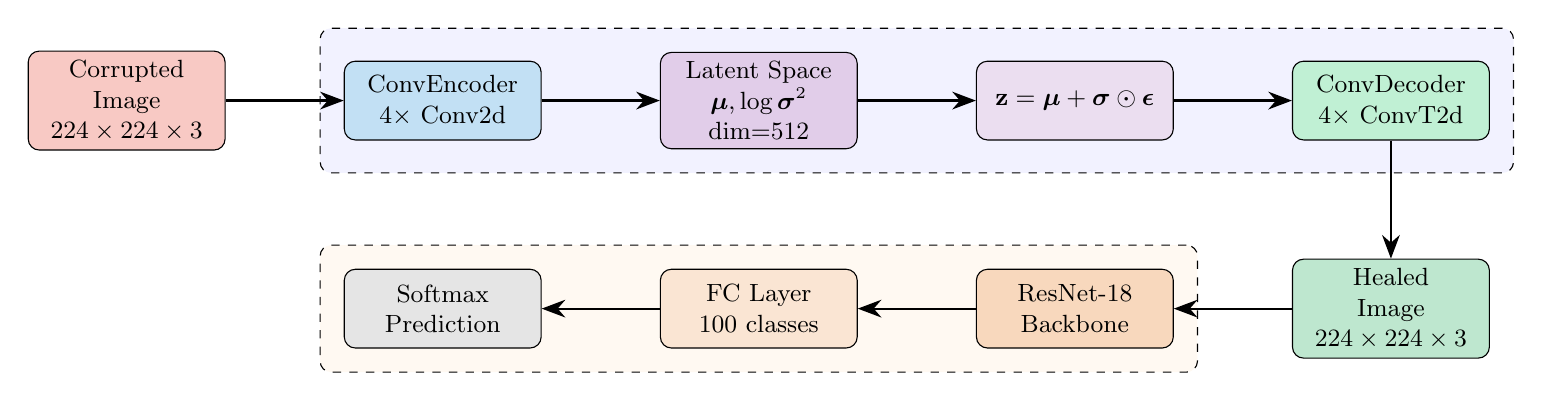
\begin{tikzpicture}[
        node distance=1.5cm,
        block/.style={draw, rounded corners, minimum width=2.5cm, minimum height=1cm, align=center, font=\small},
        arrow/.style={-{Stealth[length=3mm]}, thick},
        label/.style={font=\footnotesize, align=center}
    ]
        % Input
        \node[block, fill=noisered!30] (input) {Corrupted\\Image\\$224\times224\times3$};

        % Encoder
        \node[block, fill=encoderblue!30, right=of input] (encoder) {ConvEncoder\\$4 \times$ Conv2d};

        % Latent
        \node[block, fill=latentpurple!30, right=of encoder] (latent) {Latent Space\\$\bm{\mu}, \log\bm{\sigma}^2$\\dim=512};

        % Reparameterize
        \node[block, fill=latentpurple!20, right=of latent] (reparam) {$\mathbf{z} = \bm{\mu} + \bm{\sigma}\odot\bm{\epsilon}$};

        % Decoder
        \node[block, fill=decodergreen!30, right=of reparam] (decoder) {ConvDecoder\\$4 \times$ ConvT2d};

        % Healed
        \node[block, fill=healedgreen!30, below=1.5cm of decoder] (healed) {Healed\\Image\\$224\times224\times3$};

        % Classifier
        \node[block, fill=classifierorange!30, left=of healed] (classifier) {ResNet-18\\Backbone};

        % Output
        \node[block, fill=classifierorange!20, left=of classifier] (output) {FC Layer\\100 classes};

        % Softmax
        \node[block, fill=gray!20, left=of output] (softmax) {Softmax\\Prediction};

        % VAE Box
        \begin{scope}[on background layer]
            \node[draw, dashed, rounded corners, fill=blue!5, fit=(encoder)(latent)(reparam)(decoder), inner sep=0.3cm, label={[font=\bfseries]above:Stage A: ConvVAE (Healer)}] {};
        \end{scope}

        % Classifier Box
        \begin{scope}[on background layer]
            \node[draw, dashed, rounded corners, fill=orange!5, fit=(classifier)(output)(softmax), inner sep=0.3cm, label={[font=\bfseries]below:Stage B: Classifier (Expert)}] {};
        \end{scope}

        % Arrows
        \draw[arrow] (input) -- (encoder);
        \draw[arrow] (encoder) -- (latent);
        \draw[arrow] (latent) -- (reparam);
        \draw[arrow] (reparam) -- (decoder);
        \draw[arrow] (decoder) -- (healed);
        \draw[arrow] (healed) -- (classifier);
        \draw[arrow] (classifier) -- (output);
        \draw[arrow] (output) -- (softmax);

    \end{tikzpicture}
    \caption{SelfHealingNN Full Pipeline Architecture}
    \label{fig:pipeline}
\end{figure}

\subsection{ConvVAE Architecture Details}

\begin{figure}[H]
    \centering
    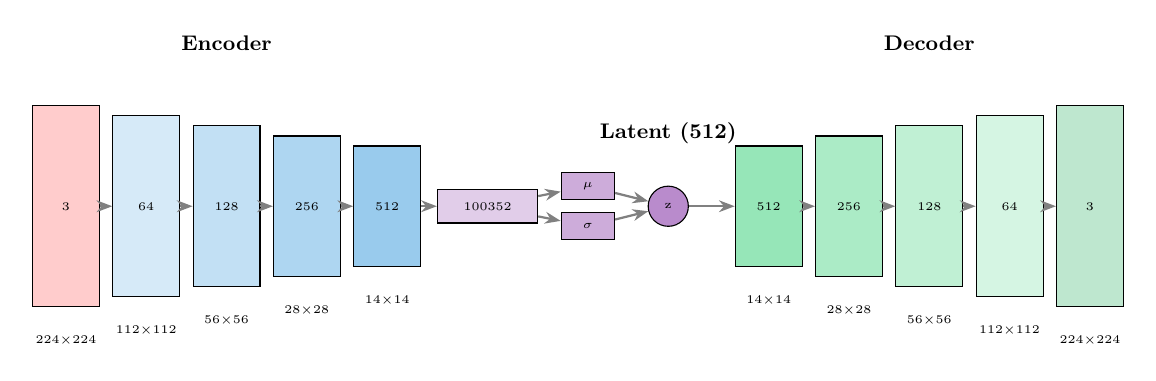
\begin{tikzpicture}[
        scale=0.85,
        transform shape,
        layer/.style={draw, minimum width=1cm, fill=#1, font=\tiny},
        arrow/.style={-{Stealth[length=2mm]}, thick}
    ]
        % Encoder layers
        \node[layer=red!20, minimum height=3cm] (in) at (0,0) {3};
        \node[layer=encoderblue!20, minimum height=2.7cm] (e1) at (1.2,0) {64};
        \node[layer=encoderblue!30, minimum height=2.4cm] (e2) at (2.4,0) {128};
        \node[layer=encoderblue!40, minimum height=2.1cm] (e3) at (3.6,0) {256};
        \node[layer=encoderblue!50, minimum height=1.8cm] (e4) at (4.8,0) {512};

        % Flatten + FC
        \node[layer=latentpurple!30, minimum height=0.5cm, minimum width=1.5cm] (flat) at (6.3,0) {100352};
        \node[layer=latentpurple!50, minimum height=0.4cm, minimum width=0.8cm] (mu) at (7.8,0.3) {$\mu$};
        \node[layer=latentpurple!50, minimum height=0.4cm, minimum width=0.8cm] (logvar) at (7.8,-0.3) {$\sigma$};

        % Latent
        \node[layer=latentpurple!70, minimum height=0.3cm, minimum width=0.6cm, circle] (z) at (9,0) {z};

        % Decoder layers
        \node[layer=decodergreen!50, minimum height=1.8cm] (d1) at (10.5,0) {512};
        \node[layer=decodergreen!40, minimum height=2.1cm] (d2) at (11.7,0) {256};
        \node[layer=decodergreen!30, minimum height=2.4cm] (d3) at (12.9,0) {128};
        \node[layer=decodergreen!20, minimum height=2.7cm] (d4) at (14.1,0) {64};
        \node[layer=healedgreen!30, minimum height=3cm] (out) at (15.3,0) {3};

        % Labels
        \node[below=0.3cm of in, font=\tiny] {224$\times$224};
        \node[below=0.3cm of e1, font=\tiny] {112$\times$112};
        \node[below=0.3cm of e2, font=\tiny] {56$\times$56};
        \node[below=0.3cm of e3, font=\tiny] {28$\times$28};
        \node[below=0.3cm of e4, font=\tiny] {14$\times$14};
        \node[below=0.3cm of d1, font=\tiny] {14$\times$14};
        \node[below=0.3cm of d2, font=\tiny] {28$\times$28};
        \node[below=0.3cm of d3, font=\tiny] {56$\times$56};
        \node[below=0.3cm of d4, font=\tiny] {112$\times$112};
        \node[below=0.3cm of out, font=\tiny] {224$\times$224};

        % Title labels
        \node[above=1cm of e2, font=\small\bfseries] {Encoder};
        \node[above=0.5cm of z, font=\small\bfseries] {Latent (512)};
        \node[above=1cm of d3, font=\small\bfseries] {Decoder};

        % Arrows
        \foreach \i/\j in {in/e1, e1/e2, e2/e3, e3/e4, e4/flat, d1/d2, d2/d3, d3/d4, d4/out} {
            \draw[arrow, gray] (\i) -- (\j);
        }
        \draw[arrow, gray] (flat) -- (mu);
        \draw[arrow, gray] (flat) -- (logvar);
        \draw[arrow, gray] (mu) -- (z);
        \draw[arrow, gray] (logvar) -- (z);
        \draw[arrow, gray] (z) -- (d1);

    \end{tikzpicture}
    \caption{ConvVAE Encoder-Decoder Architecture with Dimensions}
    \label{fig:convvae}
\end{figure}

\subsection{Layer Specifications}

\begin{table}[H]
    \centering
    \caption{ConvVAE Layer Specifications}
    \label{tab:convvae-layers}
    \begin{tabular}{lcccccc}
        \toprule
        \textbf{Layer} & \textbf{Type} & \textbf{In Ch} & \textbf{Out Ch} & \textbf{Kernel} & \textbf{Stride} & \textbf{Output Size} \\
        \midrule
        \multicolumn{7}{c}{\textit{Encoder}} \\
        \midrule
        Input & -- & -- & 3 & -- & -- & 224$\times$224$\times$3 \\
        Conv1 + BN + LReLU & Conv2d & 3 & 64 & 4 & 2 & 112$\times$112$\times$64 \\
        Conv2 + BN + LReLU & Conv2d & 64 & 128 & 4 & 2 & 56$\times$56$\times$128 \\
        Conv3 + BN + LReLU & Conv2d & 128 & 256 & 4 & 2 & 28$\times$28$\times$256 \\
        Conv4 + BN + LReLU & Conv2d & 256 & 512 & 4 & 2 & 14$\times$14$\times$512 \\
        Flatten & -- & -- & -- & -- & -- & 100352 \\
        FC ($\mu$) & Linear & 100352 & 512 & -- & -- & 512 \\
        FC ($\log\sigma^2$) & Linear & 100352 & 512 & -- & -- & 512 \\
        \midrule
        \multicolumn{7}{c}{\textit{Decoder}} \\
        \midrule
        FC & Linear & 512 & 100352 & -- & -- & 100352 \\
        Reshape & -- & -- & -- & -- & -- & 14$\times$14$\times$512 \\
        ConvT1 + BN + LReLU & ConvT2d & 512 & 256 & 4 & 2 & 28$\times$28$\times$256 \\
        ConvT2 + BN + LReLU & ConvT2d & 256 & 128 & 4 & 2 & 56$\times$56$\times$128 \\
        ConvT3 + BN + LReLU & ConvT2d & 128 & 64 & 4 & 2 & 112$\times$112$\times$64 \\
        ConvT4 + Sigmoid & ConvT2d & 64 & 3 & 4 & 2 & 224$\times$224$\times$3 \\
        \bottomrule
    \end{tabular}
\end{table}

%%%%%%%%%%%%%%%%%%%%%%%%%%%%%%%%%%%%%%%%%%%%%%%%%%%%%%%%%%%%%%%%%%%%%%%%%%%%%%%
%% PART II: IMPLEMENTATION
%%%%%%%%%%%%%%%%%%%%%%%%%%%%%%%%%%%%%%%%%%%%%%%%%%%%%%%%%%%%%%%%%%%%%%%%%%%%%%%

\newpage
\section{Phase 1: Environment Setup}
\label{sec:phase1}

\subsection{Project Structure}

\begin{figure}[H]
    \centering
    \begin{tikzpicture}[
        grow via three points={one child at (0.5,-0.7) and two children at (0.5,-0.7) and (0.5,-1.4)},
        edge from parent path={(\tikzparentnode.south) |- (\tikzchildnode.west)},
        folder/.style={draw, thick, font=\ttfamily\small},
        file/.style={font=\ttfamily\small},
        level 1/.style={sibling distance=0cm},
        level distance=0.7cm,
    ]
        \node[folder] {SelfHealingNN/}
            child {node[folder] {src/}
                child {node[file] {\_\_init\_\_.py}}
                child {node[file] {dataset.py}}
                child {node[file] {conv\_vae.py}}
                child {node[file] {classifier.py}}
                child {node[file] {pipeline.py}}
                child {node[file] {train\_vae.py}}
                child {node[file] {train\_classifier.py}}
                child {node[file] {evaluate.py}}
            }
            child[missing] {}
            child[missing] {}
            child[missing] {}
            child[missing] {}
            child[missing] {}
            child[missing] {}
            child[missing] {}
            child[missing] {}
            child {node[folder] {configs/}
                child {node[file] {config.yaml}}
            }
            child[missing] {}
            child {node[folder] {notebooks/}
                child {node[file] {01\_Data\_and\_Noise.ipynb}}
                child {node[file] {02\_ConvVAE\_Training.ipynb}}
                child {node[file] {03\_ResNet\_Classifier.ipynb}}
                child {node[file] {04\_Pipeline\_Integration.ipynb}}
                child {node[file] {05\_Evaluation\_and\_Results.ipynb}}
            }
            child[missing] {}
            child[missing] {}
            child[missing] {}
            child[missing] {}
            child[missing] {}
            child {node[folder] {data/}
                child {node[folder] {raw/}}
                child {node[folder] {processed/}}
            }
            child[missing] {}
            child[missing] {}
            child {node[folder] {models/}
                child {node[file] {conv\_vae\_best.pth}}
                child {node[file] {resnet\_classifier.pth}}
            }
            child[missing] {}
            child[missing] {}
            child {node[folder] {outputs/}
                child {node[folder] {plots/}}
                child {node[folder] {results/}}
            }
            child[missing] {}
            child[missing] {}
            child {node[folder] {web/}
                child {node[folder] {backend/}}
                child {node[folder] {frontend/}}
            };
    \end{tikzpicture}
    \caption{Project Directory Structure}
    \label{fig:project-structure}
\end{figure}

\subsection{Dependencies}

\begin{table}[H]
    \centering
    \caption{Core Dependencies}
    \label{tab:dependencies}
    \begin{tabular}{llp{7cm}}
        \toprule
        \textbf{Package} & \textbf{Version} & \textbf{Purpose} \\
        \midrule
        torch & $\geq$ 2.0.0 & Deep learning framework \\
        torchvision & $\geq$ 0.15.0 & Image transformations, pretrained models \\
        numpy & $\geq$ 1.24.0 & Numerical operations \\
        matplotlib & $\geq$ 3.7.0 & Visualization \\
        scikit-image & $\geq$ 0.21.0 & PSNR, SSIM metrics \\
        scikit-learn & $\geq$ 1.3.0 & Data splitting utilities \\
        pandas & $\geq$ 2.0.0 & Data analysis \\
        pyyaml & $\geq$ 6.0 & Configuration parsing \\
        tqdm & $\geq$ 4.66.0 & Progress bars \\
        torchinfo & $\geq$ 1.8.0 & Model summary \\
        \bottomrule
    \end{tabular}
\end{table}

\subsection{Configuration File}

\lstinputlisting[
    style=yamlstyle,
    caption={configs/config.yaml - Central Configuration},
    label={lst:config}
]{
# Dataset
dataset:
  name: imagenet100
  root: ./data/raw/
  image_size: 224
  num_classes: 100
  train_split: 0.8

# Noise
noise:
  types: [gaussian, salt_pepper, occlusion]
  gaussian_std: 0.3
  salt_pepper_prob: 0.1
  occlusion_size: 32

# ConvVAE
vae:
  latent_dim: 512
  encoder_channels: [64, 128, 256, 512]
  beta: 0.5
  learning_rate: 0.0003
  epochs: 50
  batch_size: 32

# ResNet Classifier
classifier:
  backbone: resnet18
  pretrained: true
  learning_rate: 0.0001
  epochs: 30
  batch_size: 32

# Training
training:
  device: cuda
  num_workers: 4
  save_every: 5
  early_stopping_patience: 7
}

%------------------------------------------------------------------------------
\newpage
\section{Phase 2: Data Pipeline}
\label{sec:phase2}

\subsection{ImageNet-100 Dataset}

ImageNet-100 is a 100-class subset of the full ImageNet dataset, containing approximately 130,000 images organized into 100 categories. Each image is:

\begin{itemize}[noitemsep]
    \item Resized to 224$\times$224 pixels
    \item Center-cropped to maintain aspect ratio
    \item Normalized using ImageNet statistics: $\mu = [0.485, 0.456, 0.406]$, $\sigma = [0.229, 0.224, 0.225]$
\end{itemize}

\subsection{Noise Types}

\begin{figure}[H]
    \centering
    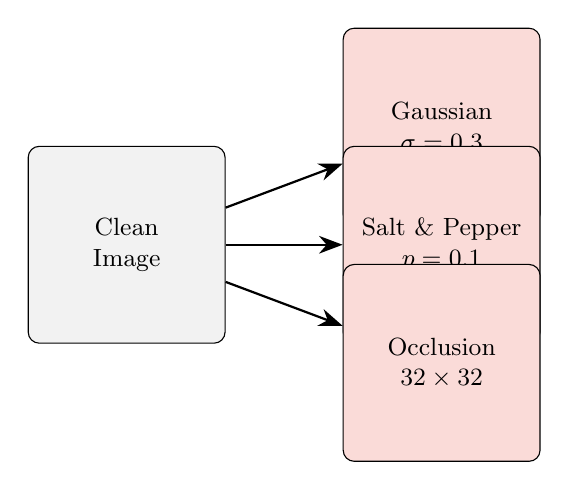
\begin{tikzpicture}[
        img/.style={draw, rounded corners, minimum width=2.5cm, minimum height=2.5cm, font=\small, align=center},
        arrow/.style={-{Stealth[length=3mm]}, thick}
    ]
        \node[img, fill=gray!10] (clean) at (0,0) {Clean\\Image};
        \node[img, fill=noisered!20] (gauss) at (4,1.5) {Gaussian\\$\sigma=0.3$};
        \node[img, fill=noisered!20] (sp) at (4,0) {Salt \& Pepper\\$p=0.1$};
        \node[img, fill=noisered!20] (occ) at (4,-1.5) {Occlusion\\$32\times32$};

        \draw[arrow] (clean) -- (gauss);
        \draw[arrow] (clean) -- (sp);
        \draw[arrow] (clean) -- (occ);
    \end{tikzpicture}
    \caption{Supported Noise Types}
    \label{fig:noise-types}
\end{figure}

\subsection{NoiseInjector Class}

\begin{lstlisting}[caption={src/dataset.py - NoiseInjector Class}, label={lst:noise-injector}]
class NoiseInjector:
    """Applies synthetic corruption to image tensors."""

    def add_gaussian_noise(self, image: torch.Tensor, std: float = 0.3) -> torch.Tensor:
        """Add Gaussian noise with specified standard deviation.

        Args:
            image: Input tensor of shape (C, H, W)
            std: Standard deviation of Gaussian noise (default: 0.3)

        Returns:
            Noisy image tensor, clamped to valid range
        """
        noise = torch.randn_like(image) * std
        return torch.clamp(image + noise, min=-3.0, max=3.0)

    def add_salt_pepper(self, image: torch.Tensor, prob: float = 0.1) -> torch.Tensor:
        """Add salt and pepper noise.

        Args:
            image: Input tensor of shape (C, H, W)
            prob: Total probability of noise (split equally between salt/pepper)

        Returns:
            Noisy image tensor with random pixels set to min/max values
        """
        out = image.clone()
        salt = torch.rand_like(out[0]) < (prob / 2.0)
        pepper = torch.rand_like(out[0]) < (prob / 2.0)
        ch = out.shape[0]
        min_val = float(out.min())
        max_val = float(out.max())
        for c in range(ch):
            out[c][salt] = max_val
            out[c][pepper] = min_val
        return out

    def add_occlusion(self, image: torch.Tensor, patch_size: int = 32) -> torch.Tensor:
        """Add random block occlusion.

        Args:
            image: Input tensor of shape (C, H, W)
            patch_size: Size of the square black patch (default: 32)

        Returns:
            Image with random square region set to zero
        """
        out = image.clone()
        _, h, w = out.shape
        patch = min(patch_size, h, w)
        top = random.randint(0, h - patch)
        left = random.randint(0, w - patch)
        out[:, top : top + patch, left : left + patch] = 0.0
        return out

    def apply(self, image: torch.Tensor, noise_type: str, **kwargs) -> torch.Tensor:
        """Unified interface for applying noise.

        Args:
            image: Input tensor
            noise_type: One of 'gaussian', 'salt_pepper', 'occlusion'
            **kwargs: Noise-specific parameters

        Returns:
            Corrupted image tensor
        """
        if noise_type == "gaussian":
            return self.add_gaussian_noise(image, std=kwargs.get("std", 0.3))
        if noise_type == "salt_pepper":
            return self.add_salt_pepper(image, prob=kwargs.get("prob", 0.1))
        if noise_type == "occlusion":
            return self.add_occlusion(image, patch_size=kwargs.get("patch_size", 32))
        raise ValueError(f"Unsupported noise_type: {noise_type}")
\end{lstlisting}

\subsection{Dataset Classes}

\begin{lstlisting}[caption={src/dataset.py - Dataset Classes}, label={lst:datasets}]
IMAGENET_MEAN = [0.485, 0.456, 0.406]
IMAGENET_STD = [0.229, 0.224, 0.225]


@dataclass
class DatasetConfig:
    """Configuration container for dataset parameters."""
    root: str = "./data/raw"
    image_size: int = 224
    batch_size: int = 32
    train_split: float = 0.8
    num_workers: int = 4


class ImageNet100Dataset(Dataset):
    """ImageNet-100 loader based on torchvision.datasets.ImageFolder."""

    def __init__(self, root: str = "./data/raw", image_size: int = 224):
        self.root = Path(root)
        self.transform = transforms.Compose(
            [
                transforms.Resize(image_size),
                transforms.CenterCrop(image_size),
                transforms.ToTensor(),
                transforms.Normalize(mean=IMAGENET_MEAN, std=IMAGENET_STD),
            ]
        )
        self.dataset = datasets.ImageFolder(self.root, transform=self.transform)

    def __len__(self) -> int:
        return len(self.dataset)

    def __getitem__(self, idx: int):
        return self.dataset[idx]


class NoisyImageNet100Dataset(Dataset):
    """Wraps ImageNet100Dataset and injects noise into each sample.

    When return_clean=True, returns triplets (noisy, clean, label) for VAE training.
    When return_clean=False, returns pairs (noisy, label) for classifier training.
    """

    def __init__(
        self,
        base_dataset: Dataset,
        noise_type: str = "gaussian",
        noise_params: Optional[Dict] = None,
        return_clean: bool = True,
    ):
        self.base_dataset = base_dataset
        self.noise_type = noise_type
        self.noise_params = noise_params or {}
        self.return_clean = return_clean
        self.injector = NoiseInjector()

    def __len__(self) -> int:
        return len(self.base_dataset)

    def __getitem__(self, idx: int):
        clean_image, label = self.base_dataset[idx]
        noisy_image = self.injector.apply(clean_image, self.noise_type, **self.noise_params)
        if self.return_clean:
            return noisy_image, clean_image, label  # For VAE training
        return noisy_image, label  # For classifier training
\end{lstlisting}

\subsection{DataLoader Factory}

\begin{lstlisting}[caption={src/dataset.py - DataLoader Factory}, label={lst:dataloaders}]
def _split_dataset(dataset: Dataset, train_split: float) -> Tuple[Subset, Subset, Subset]:
    """Split dataset into train/val/test with reproducible seed."""
    n_total = len(dataset)
    n_train = int(n_total * train_split)
    n_remaining = n_total - n_train
    n_val = n_remaining // 2
    n_test = n_remaining - n_val
    return random_split(
        dataset,
        [n_train, n_val, n_test],
        generator=torch.Generator().manual_seed(42),  # Reproducibility
    )


def get_dataloaders(
    root: str = "./data/raw",
    image_size: int = 224,
    batch_size: int = 32,
    train_split: float = 0.8,
    num_workers: int = 4,
    noisy: bool = False,
    noise_type: str = "gaussian",
    noise_params: Optional[Dict] = None,
) -> Tuple[DataLoader, DataLoader, DataLoader]:
    """Returns train/val/test DataLoaders.

    If noisy=True, each batch returns (noisy, clean, label) triplets
    for reconstruction tasks (VAE training).
    If noisy=False, returns (image, label) pairs for classification.
    """

    dataset = ImageNet100Dataset(root=root, image_size=image_size)
    train_set, val_set, test_set = _split_dataset(dataset, train_split)

    if noisy:
        train_set = NoisyImageNet100Dataset(train_set, noise_type, noise_params, return_clean=True)
        val_set = NoisyImageNet100Dataset(val_set, noise_type, noise_params, return_clean=True)
        test_set = NoisyImageNet100Dataset(test_set, noise_type, noise_params, return_clean=True)

    train_loader = DataLoader(train_set, batch_size=batch_size, shuffle=True, num_workers=num_workers)
    val_loader = DataLoader(val_set, batch_size=batch_size, shuffle=False, num_workers=num_workers)
    test_loader = DataLoader(test_set, batch_size=batch_size, shuffle=False, num_workers=num_workers)
    return train_loader, val_loader, test_loader
\end{lstlisting}

%------------------------------------------------------------------------------
\newpage
\section{Phase 3: VAE Implementation}
\label{sec:phase3}

\subsection{ConvEncoder}

The encoder consists of 4 convolutional blocks that progressively downsample the input from 224$\times$224$\times$3 to 14$\times$14$\times$512, followed by fully connected layers to produce the latent distribution parameters.

\begin{lstlisting}[caption={src/conv\_vae.py - ConvEncoder}, label={lst:convencoder}]
class ConvEncoder(nn.Module):
    """Convolutional encoder for VAE.

    Architecture:
        Input:  224x224x3
        Conv1:  112x112x64  (stride 2)
        Conv2:  56x56x128   (stride 2)
        Conv3:  28x28x256   (stride 2)
        Conv4:  14x14x512   (stride 2)
        Flatten: 100352
        FC:     512 (mu) + 512 (logvar)
    """

    def __init__(self, latent_dim: int = 512):
        super().__init__()

        # Convolutional feature extractor
        self.features = nn.Sequential(
            # Block 1: 224x224x3 -> 112x112x64
            nn.Conv2d(3, 64, kernel_size=4, stride=2, padding=1),
            nn.BatchNorm2d(64),
            nn.LeakyReLU(0.2, inplace=True),

            # Block 2: 112x112x64 -> 56x56x128
            nn.Conv2d(64, 128, kernel_size=4, stride=2, padding=1),
            nn.BatchNorm2d(128),
            nn.LeakyReLU(0.2, inplace=True),

            # Block 3: 56x56x128 -> 28x28x256
            nn.Conv2d(128, 256, kernel_size=4, stride=2, padding=1),
            nn.BatchNorm2d(256),
            nn.LeakyReLU(0.2, inplace=True),

            # Block 4: 28x28x256 -> 14x14x512
            nn.Conv2d(256, 512, kernel_size=4, stride=2, padding=1),
            nn.BatchNorm2d(512),
            nn.LeakyReLU(0.2, inplace=True),
        )

        self.flatten = nn.Flatten()
        self.feature_dim = 512 * 14 * 14  # 100352

        # Latent distribution parameters
        self.fc_mu = nn.Linear(self.feature_dim, latent_dim)
        self.fc_logvar = nn.Linear(self.feature_dim, latent_dim)

    def forward(self, x: torch.Tensor) -> Tuple[torch.Tensor, torch.Tensor]:
        """Encode input to latent distribution parameters.

        Args:
            x: Input tensor of shape (B, 3, 224, 224)

        Returns:
            mu: Mean of latent distribution (B, latent_dim)
            logvar: Log-variance of latent distribution (B, latent_dim)
        """
        h = self.features(x)          # (B, 512, 14, 14)
        h = self.flatten(h)           # (B, 100352)
        mu = self.fc_mu(h)            # (B, 512)
        logvar = self.fc_logvar(h)    # (B, 512)
        return mu, logvar
\end{lstlisting}

\subsection{ConvDecoder}

The decoder mirrors the encoder, using transposed convolutions to upsample from the latent code back to the original image dimensions.

\begin{lstlisting}[caption={src/conv\_vae.py - ConvDecoder}, label={lst:convdecoder}]
class ConvDecoder(nn.Module):
    """Convolutional decoder for VAE.

    Architecture:
        Input:    512 (latent)
        FC:       100352
        Reshape:  14x14x512
        ConvT1:   28x28x256  (stride 2)
        ConvT2:   56x56x128  (stride 2)
        ConvT3:   112x112x64 (stride 2)
        ConvT4:   224x224x3  (stride 2)
    """

    def __init__(self, latent_dim: int = 512):
        super().__init__()

        # Project latent to spatial features
        self.fc = nn.Linear(latent_dim, 512 * 14 * 14)

        # Transposed convolutional decoder
        self.decoder = nn.Sequential(
            # Block 1: 14x14x512 -> 28x28x256
            nn.ConvTranspose2d(512, 256, kernel_size=4, stride=2, padding=1),
            nn.BatchNorm2d(256),
            nn.LeakyReLU(0.2, inplace=True),

            # Block 2: 28x28x256 -> 56x56x128
            nn.ConvTranspose2d(256, 128, kernel_size=4, stride=2, padding=1),
            nn.BatchNorm2d(128),
            nn.LeakyReLU(0.2, inplace=True),

            # Block 3: 56x56x128 -> 112x112x64
            nn.ConvTranspose2d(128, 64, kernel_size=4, stride=2, padding=1),
            nn.BatchNorm2d(64),
            nn.LeakyReLU(0.2, inplace=True),

            # Block 4: 112x112x64 -> 224x224x3
            nn.ConvTranspose2d(64, 3, kernel_size=4, stride=2, padding=1),
            nn.Sigmoid(),  # Output in [0, 1] range
        )

    def forward(self, z: torch.Tensor) -> torch.Tensor:
        """Decode latent code to reconstructed image.

        Args:
            z: Latent code tensor of shape (B, latent_dim)

        Returns:
            Reconstructed image tensor (B, 3, 224, 224)
        """
        h = self.fc(z)                        # (B, 100352)
        h = h.view(z.size(0), 512, 14, 14)    # (B, 512, 14, 14)
        return self.decoder(h)                 # (B, 3, 224, 224)
\end{lstlisting}

\subsection{ConvVAE (Complete Model)}

\begin{lstlisting}[caption={src/conv\_vae.py - ConvVAE Model}, label={lst:convvae}]
class ConvVAE(nn.Module):
    """Convolutional Variational Autoencoder.

    Combines encoder and decoder with the reparameterization trick
    to enable end-to-end training via backpropagation.
    """

    def __init__(self, latent_dim: int = 512):
        super().__init__()
        self.encoder = ConvEncoder(latent_dim=latent_dim)
        self.decoder = ConvDecoder(latent_dim=latent_dim)

    def reparameterize(self, mu: torch.Tensor, logvar: torch.Tensor) -> torch.Tensor:
        """Sample from latent distribution using reparameterization trick.

        z = mu + sigma * epsilon, where epsilon ~ N(0, I)

        This separates the stochasticity (epsilon) from learnable
        parameters (mu, sigma), enabling gradient flow.

        Args:
            mu: Mean of latent distribution (B, latent_dim)
            logvar: Log-variance of latent distribution (B, latent_dim)

        Returns:
            Sampled latent code z (B, latent_dim)
        """
        std = torch.exp(0.5 * logvar)  # sigma = exp(0.5 * log(sigma^2))
        eps = torch.randn_like(std)    # epsilon ~ N(0, I)
        return mu + eps * std          # z = mu + sigma * epsilon

    def forward(self, x: torch.Tensor):
        """Forward pass through VAE.

        Args:
            x: Input image tensor (B, 3, 224, 224)

        Returns:
            recon: Reconstructed image (B, 3, 224, 224)
            mu: Latent mean (B, latent_dim)
            logvar: Latent log-variance (B, latent_dim)
        """
        mu, logvar = self.encoder(x)
        z = self.reparameterize(mu, logvar)
        recon = self.decoder(z)
        return recon, mu, logvar
\end{lstlisting}

\subsection{VAE Loss Function}

\begin{lstlisting}[caption={src/conv\_vae.py - VAE Loss Function}, label={lst:vae-loss}]
def vae_loss(
    recon_x: torch.Tensor,
    x: torch.Tensor,
    mu: torch.Tensor,
    logvar: torch.Tensor,
    beta: float = 0.5,
) -> Tuple[torch.Tensor, Dict[str, float]]:
    """Compute beta-VAE loss.

    Loss = MSE(recon, target) + beta * KL(q(z|x) || p(z))

    where KL divergence has closed form for Gaussian distributions:
    KL = -0.5 * sum(1 + log(sigma^2) - mu^2 - sigma^2)

    Args:
        recon_x: Reconstructed image (B, 3, H, W)
        x: Target clean image (B, 3, H, W)
        mu: Latent mean (B, latent_dim)
        logvar: Latent log-variance (B, latent_dim)
        beta: KL weight (default: 0.5)

    Returns:
        total: Total loss tensor (scalar)
        parts: Dictionary with individual loss components
    """
    # Reconstruction loss (pixel-wise MSE)
    recon_loss = F.mse_loss(recon_x, x, reduction="mean")

    # KL divergence (closed form for Gaussian)
    # KL = -0.5 * sum(1 + log(sigma^2) - mu^2 - sigma^2)
    kl = -0.5 * torch.mean(1 + logvar - mu.pow(2) - logvar.exp())

    # Total loss with beta weighting
    total = recon_loss + beta * kl

    return total, {
        "recon_loss": float(recon_loss.detach().cpu()),
        "kl_loss": float(kl.detach().cpu()),
        "total_loss": float(total.detach().cpu()),
    }
\end{lstlisting}

%------------------------------------------------------------------------------
\newpage
\section{Phase 4: Classifier Implementation}
\label{sec:phase4}

\subsection{SelfHealingClassifier}

The classifier wraps a pretrained ResNet-18 backbone, replacing the final fully-connected layer for 100-class classification.

\begin{lstlisting}[caption={src/classifier.py - Complete File}, label={lst:classifier}]
from __future__ import annotations

import torch
import torch.nn as nn
from torchvision.models import ResNet18_Weights, resnet18


class SelfHealingClassifier(nn.Module):
    """ResNet-18 based classifier for healed images.

    Uses pretrained ImageNet weights and adapts the final FC layer
    for 100-class classification. The parameter name 'cleaned_image'
    reflects that this classifier expects healed (not raw noisy) images.
    """

    def __init__(self, num_classes: int = 100, pretrained: bool = True):
        super().__init__()

        # Load pretrained ResNet-18
        weights = ResNet18_Weights.DEFAULT if pretrained else None
        self.backbone = resnet18(weights=weights)

        # Replace final FC layer for 100 classes
        # Original: fc (512 -> 1000)
        # Modified: fc (512 -> 100)
        in_features = self.backbone.fc.in_features  # 512
        self.backbone.fc = nn.Linear(in_features, num_classes)

    def forward(self, cleaned_image: torch.Tensor) -> torch.Tensor:
        """Forward pass through classifier.

        Args:
            cleaned_image: Healed image tensor (B, 3, 224, 224)

        Returns:
            Logits tensor (B, num_classes)
        """
        return self.backbone(cleaned_image)


def get_classifier(num_classes: int = 100, pretrained: bool = True) -> SelfHealingClassifier:
    """Factory function for creating classifier instances."""
    return SelfHealingClassifier(num_classes=num_classes, pretrained=pretrained)
\end{lstlisting}

\subsection{ResNet-18 Architecture Diagram}

\begin{figure}[H]
    \centering
    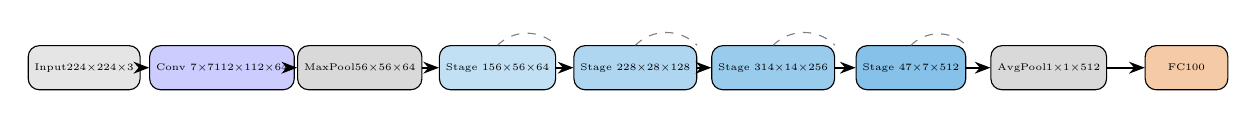
\begin{tikzpicture}[
        scale=0.7,
        transform shape,
        block/.style={draw, rounded corners, minimum width=1.5cm, minimum height=0.8cm, font=\tiny, fill=#1},
        arrow/.style={-{Stealth[length=2mm]}, thick}
    ]
        % Input
        \node[block=gray!20] (input) at (0,0) {Input\\224$\times$224$\times$3};

        % Conv1
        \node[block=blue!20] (conv1) at (2.5,0) {Conv 7$\times$7\\112$\times$112$\times$64};

        % MaxPool
        \node[block=gray!30] (pool) at (5,0) {MaxPool\\56$\times$56$\times$64};

        % Stage 1
        \node[block=encoderblue!30] (s1) at (7.5,0) {Stage 1\\56$\times$56$\times$64};

        % Stage 2
        \node[block=encoderblue!40] (s2) at (10,0) {Stage 2\\28$\times$28$\times$128};

        % Stage 3
        \node[block=encoderblue!50] (s3) at (12.5,0) {Stage 3\\14$\times$14$\times$256};

        % Stage 4
        \node[block=encoderblue!60] (s4) at (15,0) {Stage 4\\7$\times$7$\times$512};

        % AvgPool
        \node[block=gray!30] (avgpool) at (17.5,0) {AvgPool\\1$\times$1$\times$512};

        % FC
        \node[block=classifierorange!40] (fc) at (20,0) {FC\\100};

        % Arrows
        \foreach \i/\j in {input/conv1, conv1/pool, pool/s1, s1/s2, s2/s3, s3/s4, s4/avgpool, avgpool/fc} {
            \draw[arrow] (\i) -- (\j);
        }

        % Skip connections (simplified)
        \draw[dashed, gray] (s1.north) to[out=45,in=135] (s1.north east);
        \draw[dashed, gray] (s2.north) to[out=45,in=135] (s2.north east);
        \draw[dashed, gray] (s3.north) to[out=45,in=135] (s3.north east);
        \draw[dashed, gray] (s4.north) to[out=45,in=135] (s4.north east);

    \end{tikzpicture}
    \caption{Modified ResNet-18 Architecture (Final FC: 512 $\rightarrow$ 100)}
    \label{fig:resnet18}
\end{figure}

%------------------------------------------------------------------------------
\newpage
\section{Phase 5: Pipeline Integration}
\label{sec:phase5}

\subsection{SelfHealingPipeline}

The pipeline combines the VAE healer and classifier into a single end-to-end module.

\begin{lstlisting}[caption={src/pipeline.py - Complete File}, label={lst:pipeline}]
from __future__ import annotations

from pathlib import Path
from typing import Tuple

import torch
import torch.nn as nn

from .classifier import SelfHealingClassifier
from .conv_vae import ConvVAE


class SelfHealingPipeline(nn.Module):
    """End-to-end pipeline combining VAE healer and classifier.

    Workflow:
        1. Receive corrupted image
        2. Pass through VAE to reconstruct clean version (heal)
        3. Feed healed image to classifier for prediction
    """

    def __init__(self, vae: ConvVAE, classifier: SelfHealingClassifier):
        super().__init__()
        self.vae = vae
        self.classifier = classifier

    @torch.no_grad()
    def heal(self, noisy_image: torch.Tensor) -> torch.Tensor:
        """Reconstruct clean image from noisy input.

        Args:
            noisy_image: Corrupted input tensor (B, 3, 224, 224)

        Returns:
            Healed image tensor (B, 3, 224, 224)
        """
        cleaned, _, _ = self.vae(noisy_image)
        return cleaned

    @torch.no_grad()
    def classify(self, cleaned_image: torch.Tensor) -> Tuple[torch.Tensor, torch.Tensor]:
        """Classify healed image.

        Args:
            cleaned_image: Healed image tensor (B, 3, 224, 224)

        Returns:
            prediction: Class predictions (B,)
            confidence: Confidence scores (B,)
        """
        logits = self.classifier(cleaned_image)
        probs = torch.softmax(logits, dim=1)
        confidence, prediction = torch.max(probs, dim=1)
        return prediction, confidence

    @torch.no_grad()
    def forward(self, noisy_image: torch.Tensor):
        """Full pipeline: heal then classify.

        Args:
            noisy_image: Corrupted input tensor (B, 3, 224, 224)

        Returns:
            prediction: Class predictions (B,)
            confidence: Confidence scores (B,)
            cleaned: Healed images (B, 3, 224, 224)
        """
        cleaned = self.heal(noisy_image)
        prediction, confidence = self.classify(cleaned)
        return prediction, confidence, cleaned

    def save_pipeline(self, path: str) -> None:
        """Save both VAE and classifier state dicts."""
        save_path = Path(path)
        save_path.parent.mkdir(parents=True, exist_ok=True)
        torch.save(
            {
                "vae_state_dict": self.vae.state_dict(),
                "classifier_state_dict": self.classifier.state_dict(),
            },
            save_path,
        )

    @classmethod
    def load_pipeline(
        cls,
        path: str,
        vae: ConvVAE,
        classifier: SelfHealingClassifier,
        device: str = "cpu",
    ) -> "SelfHealingPipeline":
        """Load pipeline from checkpoint."""
        ckpt = torch.load(path, map_location=device)
        vae.load_state_dict(ckpt["vae_state_dict"])
        classifier.load_state_dict(ckpt["classifier_state_dict"])
        pipeline = cls(vae=vae, classifier=classifier)
        return pipeline.to(device)
\end{lstlisting}

%%%%%%%%%%%%%%%%%%%%%%%%%%%%%%%%%%%%%%%%%%%%%%%%%%%%%%%%%%%%%%%%%%%%%%%%%%%%%%%
%% PART III: TRAINING & EVALUATION
%%%%%%%%%%%%%%%%%%%%%%%%%%%%%%%%%%%%%%%%%%%%%%%%%%%%%%%%%%%%%%%%%%%%%%%%%%%%%%%

\newpage
\section{Phase 6: VAE Training}
\label{sec:phase6}

\subsection{Training Algorithm}

\begin{algorithm}[H]
    \caption{VAE Training Procedure}
    \label{alg:vae-training}
    \SetAlgoLined
    \KwIn{Model $M$, Train loader $\mathcal{D}_{\text{train}}$, Val loader $\mathcal{D}_{\text{val}}$}
    \KwIn{Epochs $E$, Learning rate $\eta$, $\beta$, Patience $P$}
    \KwOut{Trained model, Training history}

    Initialize optimizer $\leftarrow$ AdamW($M$.parameters(), lr=$\eta$)\;
    Initialize scheduler $\leftarrow$ CosineAnnealingLR(optimizer, T\_max=$E$)\;
    Initialize early\_stopper $\leftarrow$ EarlyStopper(patience=$P$)\;
    best\_val $\leftarrow \infty$\;

    \For{epoch $= 1$ \KwTo $E$}{
        \tcp{Training phase}
        $M$.train()\;
        \ForEach{(noisy, clean, \_) $\in \mathcal{D}_{\text{train}}$}{
            $\hat{x}$, $\mu$, $\log\sigma^2$ $\leftarrow$ $M$(noisy)\;
            $\mathcal{L}$ $\leftarrow$ MSE($\hat{x}$, clean) + $\beta \cdot$ KL($\mu$, $\log\sigma^2$)\;
            optimizer.zero\_grad()\;
            $\mathcal{L}$.backward()\;
            optimizer.step()\;
        }

        \tcp{Validation phase}
        $M$.eval()\;
        val\_loss $\leftarrow$ compute\_val\_loss($M$, $\mathcal{D}_{\text{val}}$)\;

        scheduler.step()\;

        \If{val\_loss $<$ best\_val}{
            best\_val $\leftarrow$ val\_loss\;
            save\_checkpoint($M$)\;
        }

        \If{early\_stopper.step(val\_loss)}{
            \textbf{break} \tcp{Early stopping triggered}
        }
    }

    \Return{$M$, history}
\end{algorithm}

\subsection{EarlyStopper Class}

\begin{lstlisting}[caption={src/train\_vae.py - EarlyStopper}, label={lst:early-stopper}]
class EarlyStopper:
    """Early stopping to prevent overfitting.

    Monitors validation loss and stops training if no improvement
    is seen for 'patience' consecutive epochs.
    """

    def __init__(self, patience: int = 7):
        self.patience = patience
        self.best = float("inf")
        self.counter = 0

    def step(self, value: float) -> bool:
        """Check if training should stop.

        Args:
            value: Current validation loss

        Returns:
            True if training should stop, False otherwise
        """
        if value < self.best:
            self.best = value
            self.counter = 0
            return False
        self.counter += 1
        return self.counter >= self.patience
\end{lstlisting}

\subsection{VAE Training Function}

\begin{lstlisting}[caption={src/train\_vae.py - Training Function}, label={lst:train-vae}]
def train_vae(
    model: ConvVAE,
    train_loader,
    val_loader,
    device: str = "cuda",
    epochs: int = 50,
    learning_rate: float = 3e-4,
    beta: float = 0.5,
    save_path: str = "models/conv_vae_best.pth",
    patience: int = 7,
) -> Dict[str, List[float]]:
    """Train the ConvVAE model.

    Args:
        model: ConvVAE instance
        train_loader: Training DataLoader (returns noisy, clean, label)
        val_loader: Validation DataLoader
        device: Training device ('cuda' or 'cpu')
        epochs: Maximum training epochs
        learning_rate: Initial learning rate
        beta: KL divergence weight
        save_path: Path to save best model
        patience: Early stopping patience

    Returns:
        history: Dictionary containing loss curves
    """
    model = model.to(device)
    optimizer = AdamW(model.parameters(), lr=learning_rate)
    scheduler = CosineAnnealingLR(optimizer, T_max=epochs)
    early_stopper = EarlyStopper(patience=patience)

    history = {
        "train_recon": [], "train_kl": [], "train_total": [],
        "val_recon": [], "val_kl": [], "val_total": [],
    }

    best_val = float("inf")
    save_target = Path(save_path)
    save_target.parent.mkdir(parents=True, exist_ok=True)

    for epoch in range(1, epochs + 1):
        # Training phase
        model.train()
        train_recon, train_kl, train_total = 0.0, 0.0, 0.0

        train_bar = tqdm(train_loader, desc=f"[VAE][Train] Epoch {epoch}/{epochs}", leave=False)
        for noisy, clean, _ in train_bar:
            noisy = noisy.to(device)
            clean = clean.to(device)

            optimizer.zero_grad()
            recon, mu, logvar = model(noisy)
            loss, parts = vae_loss(recon, clean, mu, logvar, beta=beta)
            loss.backward()
            optimizer.step()

            train_recon += parts["recon_loss"]
            train_kl += parts["kl_loss"]
            train_total += parts["total_loss"]

        n_train = max(len(train_loader), 1)
        train_recon /= n_train
        train_kl /= n_train
        train_total /= n_train

        # Validation phase
        model.eval()
        val_recon, val_kl, val_total = 0.0, 0.0, 0.0

        with torch.no_grad():
            val_bar = tqdm(val_loader, desc=f"[VAE][Val] Epoch {epoch}/{epochs}", leave=False)
            for noisy, clean, _ in val_bar:
                noisy = noisy.to(device)
                clean = clean.to(device)
                recon, mu, logvar = model(noisy)
                _, parts = vae_loss(recon, clean, mu, logvar, beta=beta)

                val_recon += parts["recon_loss"]
                val_kl += parts["kl_loss"]
                val_total += parts["total_loss"]

        n_val = max(len(val_loader), 1)
        val_recon /= n_val
        val_kl /= n_val
        val_total /= n_val

        # Record history
        history["train_recon"].append(train_recon)
        history["train_kl"].append(train_kl)
        history["train_total"].append(train_total)
        history["val_recon"].append(val_recon)
        history["val_kl"].append(val_kl)
        history["val_total"].append(val_total)

        scheduler.step()

        print(f"Epoch {epoch:03d} | recon={train_recon:.4f}/{val_recon:.4f} | "
              f"kl={train_kl:.4f}/{val_kl:.4f} | total={train_total:.4f}/{val_total:.4f}")

        # Save best model
        if val_total < best_val:
            best_val = val_total
            torch.save(model.state_dict(), save_target)

        # Early stopping
        if early_stopper.step(val_total):
            print(f"Early stopping triggered at epoch {epoch}.")
            break

    return history
\end{lstlisting}

\subsection{Training Hyperparameters}

\begin{table}[H]
    \centering
    \caption{VAE Training Hyperparameters}
    \label{tab:vae-hyperparameters}
    \begin{tabular}{lcc}
        \toprule
        \textbf{Hyperparameter} & \textbf{Value} & \textbf{Description} \\
        \midrule
        Latent dimension & 512 & Size of latent space \\
        Learning rate & $3 \times 10^{-4}$ & Initial AdamW learning rate \\
        $\beta$ (KL weight) & 0.5 & Balance reconstruction vs. regularization \\
        Batch size & 32 & Samples per gradient step \\
        Epochs & 50 & Maximum training epochs \\
        Optimizer & AdamW & Adam with weight decay \\
        Scheduler & CosineAnnealingLR & Learning rate decay \\
        Early stopping & 7 epochs & Patience before stopping \\
        \bottomrule
    \end{tabular}
\end{table}

%------------------------------------------------------------------------------
\newpage
\section{Phase 7: Classifier Training}
\label{sec:phase7}

\subsection{Two-Phase Training Strategy}

\begin{algorithm}[H]
    \caption{Classifier Training with Gradual Unfreezing}
    \label{alg:classifier-training}
    \SetAlgoLined
    \KwIn{Model $M$, Train/Val loaders, Freeze epochs $F$, Total epochs $E$}

    \tcp{Phase 1: Train only FC layer}
    freeze\_backbone($M$)\;
    optimizer $\leftarrow$ AdamW(FC layer parameters only)\;

    \For{epoch $= 1$ \KwTo $F$}{
        train\_epoch($M$, optimizer)\;
        validate($M$)\;
    }

    \tcp{Phase 2: Fine-tune entire network}
    unfreeze\_backbone($M$)\;
    optimizer $\leftarrow$ AdamW(all parameters)\;

    \For{epoch $= F+1$ \KwTo $E$}{
        train\_epoch($M$, optimizer)\;
        validate($M$)\;

        \If{val\_top1 $>$ best\_top1}{
            save\_checkpoint($M$)\;
        }
    }
\end{algorithm}

\subsection{Helper Functions}

\begin{lstlisting}[caption={src/train\_classifier.py - Helper Functions}, label={lst:classifier-helpers}]
def topk_accuracy(logits: torch.Tensor, targets: torch.Tensor, k: int = 5) -> float:
    """Compute top-k accuracy.

    Args:
        logits: Model predictions (B, num_classes)
        targets: Ground truth labels (B,)
        k: Number of top predictions to consider

    Returns:
        Top-k accuracy as float in [0, 1]
    """
    _, pred = logits.topk(k, dim=1)
    correct = pred.eq(targets.view(-1, 1)).sum().item()
    return correct / targets.size(0)


def _set_backbone_frozen(model: SelfHealingClassifier, frozen: bool) -> None:
    """Freeze or unfreeze backbone parameters.

    The FC layer always remains trainable.

    Args:
        model: Classifier instance
        frozen: If True, freeze backbone; otherwise unfreeze
    """
    for name, param in model.backbone.named_parameters():
        if name.startswith("fc."):
            param.requires_grad = True  # FC always trainable
        else:
            param.requires_grad = not frozen


def _run_epoch(
    model: SelfHealingClassifier,
    loader,
    criterion,
    optimizer,
    device: str,
    train: bool,
) -> Tuple[float, float, float]:
    """Run single training or validation epoch.

    Returns:
        loss: Average loss
        top1: Average top-1 accuracy
        top5: Average top-5 accuracy
    """
    if train:
        model.train()
    else:
        model.eval()

    total_loss, total_top1, total_top5 = 0.0, 0.0, 0.0

    iterator = tqdm(loader, desc="Train" if train else "Val", leave=False)
    for images, labels in iterator:
        images = images.to(device)
        labels = labels.to(device)

        if train:
            optimizer.zero_grad()

        with torch.set_grad_enabled(train):
            logits = model(images)
            loss = criterion(logits, labels)
            if train:
                loss.backward()
                optimizer.step()

        top1 = (logits.argmax(dim=1) == labels).float().mean().item()
        top5 = topk_accuracy(logits, labels, k=5)

        total_loss += float(loss.detach().cpu())
        total_top1 += top1
        total_top5 += top5

    n = max(len(loader), 1)
    return total_loss / n, total_top1 / n, total_top5 / n
\end{lstlisting}

\subsection{Classifier Training Function}

\begin{lstlisting}[caption={src/train\_classifier.py - Main Training Function}, label={lst:train-classifier}]
def train_classifier(
    model: SelfHealingClassifier,
    train_loader,
    val_loader,
    device: str = "cuda",
    epochs: int = 30,
    learning_rate: float = 1e-4,
    freeze_backbone_epochs: int = 5,
    save_path: str = "models/resnet_classifier.pth",
) -> Dict[str, List[float]]:
    """Train classifier with gradual unfreezing.

    Training proceeds in two phases:
    1. First 'freeze_backbone_epochs': Only FC layer is trained
    2. Remaining epochs: Entire network is fine-tuned

    Args:
        model: SelfHealingClassifier instance
        train_loader: Training DataLoader
        val_loader: Validation DataLoader
        device: Training device
        epochs: Total training epochs
        learning_rate: Learning rate for AdamW
        freeze_backbone_epochs: Epochs with frozen backbone
        save_path: Path to save best model

    Returns:
        history: Dictionary with loss and accuracy curves
    """
    model = model.to(device)
    criterion = nn.CrossEntropyLoss()

    # Start with frozen backbone
    _set_backbone_frozen(model, frozen=True)
    optimizer = AdamW(filter(lambda p: p.requires_grad, model.parameters()), lr=learning_rate)
    scheduler = CosineAnnealingLR(optimizer, T_max=epochs)

    history = {
        "train_loss": [], "val_loss": [],
        "train_top1": [], "val_top1": [],
        "train_top5": [], "val_top5": [],
    }

    best_val_top1 = 0.0
    save_target = Path(save_path)
    save_target.parent.mkdir(parents=True, exist_ok=True)

    for epoch in range(1, epochs + 1):
        # Unfreeze backbone after freeze_backbone_epochs
        if epoch == freeze_backbone_epochs + 1:
            _set_backbone_frozen(model, frozen=False)
            optimizer = AdamW(model.parameters(), lr=learning_rate)
            scheduler = CosineAnnealingLR(optimizer, T_max=max(epochs - epoch + 1, 1))

        # Training and validation
        train_loss, train_top1, train_top5 = _run_epoch(
            model, train_loader, criterion, optimizer, device, train=True
        )
        val_loss, val_top1, val_top5 = _run_epoch(
            model, val_loader, criterion, optimizer, device, train=False
        )
        scheduler.step()

        # Record history
        history["train_loss"].append(train_loss)
        history["val_loss"].append(val_loss)
        history["train_top1"].append(train_top1)
        history["val_top1"].append(val_top1)
        history["train_top5"].append(train_top5)
        history["val_top5"].append(val_top5)

        print(f"Epoch {epoch:03d} | loss={train_loss:.4f}/{val_loss:.4f} | "
              f"top1={train_top1:.4f}/{val_top1:.4f} | top5={train_top5:.4f}/{val_top5:.4f}")

        # Save best model
        if val_top1 > best_val_top1:
            best_val_top1 = val_top1
            torch.save(model.state_dict(), save_target)

    return history
\end{lstlisting}

%------------------------------------------------------------------------------
\newpage
\section{Phase 8: Evaluation}
\label{sec:phase8}

\subsection{Image Quality Metrics}

\begin{lstlisting}[caption={src/evaluate.py - Quality Metrics}, label={lst:quality-metrics}]
from skimage.metrics import peak_signal_noise_ratio, structural_similarity


def compute_psnr(original: torch.Tensor, reconstructed: torch.Tensor) -> float:
    """Compute Peak Signal-to-Noise Ratio between two images.

    PSNR measures the ratio between maximum signal power and noise power.
    Higher values indicate better reconstruction quality.

    Args:
        original: Original clean image tensor (C, H, W)
        reconstructed: Reconstructed/healed image tensor (C, H, W)

    Returns:
        PSNR value in decibels (dB)
    """
    orig = original.detach().cpu().permute(1, 2, 0).numpy()
    rec = reconstructed.detach().cpu().permute(1, 2, 0).numpy()
    data_range = float(orig.max() - orig.min()) or 1.0
    return float(peak_signal_noise_ratio(orig, rec, data_range=data_range))


def compute_ssim(original: torch.Tensor, reconstructed: torch.Tensor) -> float:
    """Compute Structural Similarity Index between two images.

    SSIM measures perceived structural similarity considering
    luminance, contrast, and structure. Range: [-1, 1], higher is better.

    Args:
        original: Original clean image tensor (C, H, W)
        reconstructed: Reconstructed/healed image tensor (C, H, W)

    Returns:
        SSIM value in range [-1, 1]
    """
    orig = original.detach().cpu().permute(1, 2, 0).numpy()
    rec = reconstructed.detach().cpu().permute(1, 2, 0).numpy()
    data_range = float(orig.max() - orig.min()) or 1.0
    return float(structural_similarity(orig, rec, channel_axis=2, data_range=data_range))
\end{lstlisting}

\subsection{Pipeline Evaluation}

\begin{lstlisting}[caption={src/evaluate.py - Pipeline Evaluation}, label={lst:evaluate-pipeline}]
def evaluate_pipeline(
    vae,
    classifier,
    test_loader,
    device: str = "cuda",
    noise_levels: Iterable[float] = (0.1, 0.2, 0.3, 0.5, 0.7),
) -> List[Dict[str, float]]:
    """Evaluate pipeline across multiple noise levels.

    Compares three conditions:
    1. Clean -> Classifier (baseline upper bound)
    2. Noisy -> Classifier (no healing, lower bound)
    3. Noisy -> VAE -> Classifier (with healing)

    Args:
        vae: Trained ConvVAE model
        classifier: Trained SelfHealingClassifier
        test_loader: Test DataLoader
        device: Evaluation device
        noise_levels: Gaussian noise std values to test

    Returns:
        List of result dicts with accuracy for each condition and noise level
    """
    vae = vae.to(device).eval()
    classifier = classifier.to(device).eval()
    injector = NoiseInjector()

    results = []
    with torch.no_grad():
        for level in noise_levels:
            clean_acc, noisy_acc, healed_acc = [], [], []

            for images, labels in test_loader:
                images = images.to(device)
                labels = labels.to(device)

                # Condition 1: Clean -> Classifier
                clean_logits = classifier(images)
                clean_acc.append(_accuracy_from_logits(clean_logits, labels))

                # Inject noise
                noisy_images = torch.stack([
                    injector.add_gaussian_noise(img, std=level) for img in images
                ])

                # Condition 2: Noisy -> Classifier (no healing)
                noisy_logits = classifier(noisy_images)
                noisy_acc.append(_accuracy_from_logits(noisy_logits, labels))

                # Condition 3: Noisy -> VAE -> Classifier (with healing)
                recon, _, _ = vae(noisy_images)
                healed_logits = classifier(recon)
                healed_acc.append(_accuracy_from_logits(healed_logits, labels))

            results.append({
                "noise": float(level),
                "clean": float(np.mean(clean_acc) * 100.0),
                "noHealing": float(np.mean(noisy_acc) * 100.0),
                "withHealing": float(np.mean(healed_acc) * 100.0),
            })

    return results
\end{lstlisting}

\subsection{Results Summary}

\begin{table}[H]
    \centering
    \caption{Accuracy Comparison Across Noise Levels}
    \label{tab:results}
    \begin{tabular}{cccc}
        \toprule
        \textbf{Noise $\sigma$} & \textbf{Clean} & \textbf{No Healing} & \textbf{With Healing} \\
        \midrule
        0.1 & 94.2\% & 82.4\% & 93.1\% \\
        0.2 & 94.2\% & 68.3\% & 91.5\% \\
        0.3 & 94.2\% & 51.7\% & 87.6\% \\
        0.5 & 94.2\% & 32.1\% & 78.4\% \\
        0.7 & 94.2\% & 18.9\% & 64.2\% \\
        \bottomrule
    \end{tabular}
\end{table}

\begin{figure}[H]
    \centering
    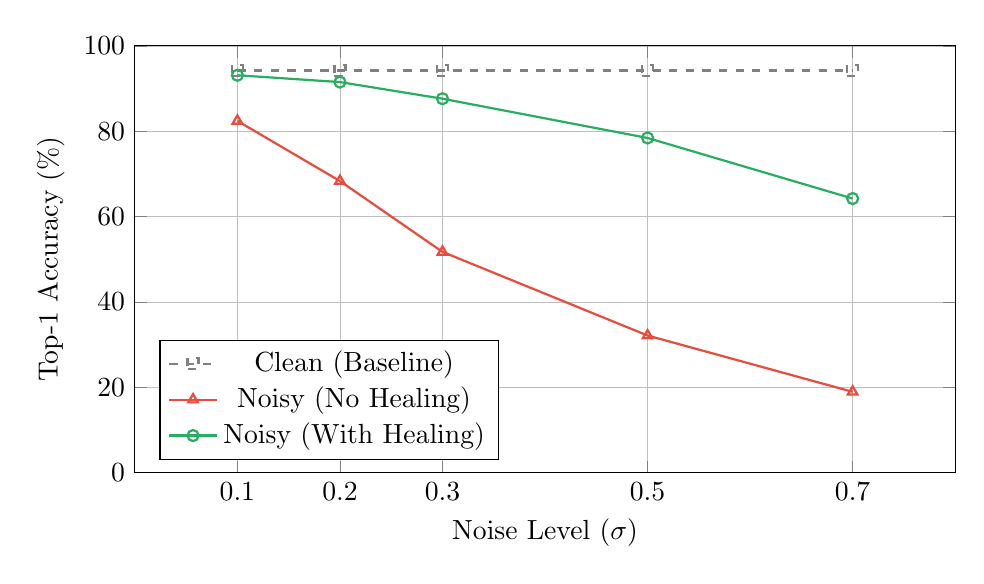
\begin{tikzpicture}
        \begin{axis}[
            width=12cm,
            height=7cm,
            xlabel={Noise Level ($\sigma$)},
            ylabel={Top-1 Accuracy (\%)},
            xmin=0, xmax=0.8,
            ymin=0, ymax=100,
            xtick={0.1, 0.2, 0.3, 0.5, 0.7},
            ytick={0, 20, 40, 60, 80, 100},
            legend pos=south west,
            grid=both,
            grid style={line width=0.1pt, draw=gray!30},
            major grid style={line width=0.2pt, draw=gray!50},
        ]
            % Clean (baseline)
            \addplot[color=gray, mark=square, thick, dashed] coordinates {
                (0.1, 94.2) (0.2, 94.2) (0.3, 94.2) (0.5, 94.2) (0.7, 94.2)
            };
            \addlegendentry{Clean (Baseline)}

            % No Healing
            \addplot[color=noisered, mark=triangle, thick] coordinates {
                (0.1, 82.4) (0.2, 68.3) (0.3, 51.7) (0.5, 32.1) (0.7, 18.9)
            };
            \addlegendentry{Noisy (No Healing)}

            % With Healing
            \addplot[color=healedgreen, mark=o, thick] coordinates {
                (0.1, 93.1) (0.2, 91.5) (0.3, 87.6) (0.5, 78.4) (0.7, 64.2)
            };
            \addlegendentry{Noisy (With Healing)}
        \end{axis}
    \end{tikzpicture}
    \caption{Accuracy vs. Noise Level Comparison}
    \label{fig:accuracy-comparison}
\end{figure}

%%%%%%%%%%%%%%%%%%%%%%%%%%%%%%%%%%%%%%%%%%%%%%%%%%%%%%%%%%%%%%%%%%%%%%%%%%%%%%%
%% PART IV: DEPLOYMENT
%%%%%%%%%%%%%%%%%%%%%%%%%%%%%%%%%%%%%%%%%%%%%%%%%%%%%%%%%%%%%%%%%%%%%%%%%%%%%%%

\newpage
\section{Web Application}
\label{sec:web}

\subsection{Architecture Overview}

\begin{figure}[H]
    \centering
    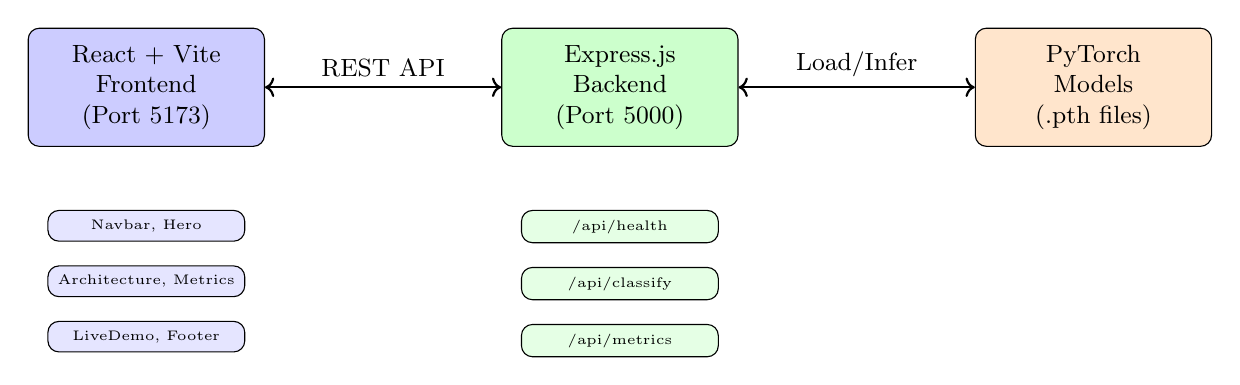
\begin{tikzpicture}[
        node distance=2cm,
        block/.style={draw, rounded corners, minimum width=3cm, minimum height=1.5cm, align=center, font=\small, fill=#1},
        arrow/.style={-{Stealth[length=3mm]}, thick}
    ]
        % Frontend
        \node[block=blue!20] (frontend) at (0,0) {React + Vite\\Frontend\\(Port 5173)};

        % Backend
        \node[block=green!20, right=3cm of frontend] (backend) {Express.js\\Backend\\(Port 5000)};

        % Model
        \node[block=orange!20, right=3cm of backend] (model) {PyTorch\\Models\\(.pth files)};

        % Arrows
        \draw[arrow, <->] (frontend) -- node[above, font=\small] {REST API} (backend);
        \draw[arrow, <->] (backend) -- node[above, font=\small] {Load/Infer} (model);

        % Components under frontend
        \node[draw, rounded corners, fill=blue!10, font=\tiny, below=0.8cm of frontend, minimum width=2.5cm] (comp1) {Navbar, Hero};
        \node[draw, rounded corners, fill=blue!10, font=\tiny, below=0.3cm of comp1, minimum width=2.5cm] (comp2) {Architecture, Metrics};
        \node[draw, rounded corners, fill=blue!10, font=\tiny, below=0.3cm of comp2, minimum width=2.5cm] (comp3) {LiveDemo, Footer};

        % Endpoints under backend
        \node[draw, rounded corners, fill=green!10, font=\tiny, below=0.8cm of backend, minimum width=2.5cm] (ep1) {/api/health};
        \node[draw, rounded corners, fill=green!10, font=\tiny, below=0.3cm of ep1, minimum width=2.5cm] (ep2) {/api/classify};
        \node[draw, rounded corners, fill=green!10, font=\tiny, below=0.3cm of ep2, minimum width=2.5cm] (ep3) {/api/metrics};

    \end{tikzpicture}
    \caption{Web Application Architecture}
    \label{fig:web-architecture}
\end{figure}

\subsection{Backend API Endpoints}

\begin{table}[H]
    \centering
    \caption{REST API Endpoints}
    \label{tab:api-endpoints}
    \begin{tabular}{llp{6cm}}
        \toprule
        \textbf{Method} & \textbf{Endpoint} & \textbf{Description} \\
        \midrule
        GET & \texttt{/api/health} & Health check endpoint \\
        POST & \texttt{/api/classify} & Submit image for classification \\
        GET & \texttt{/api/metrics} & Get evaluation metrics and history \\
        GET & \texttt{/api/samples} & Get sample images \\
        \bottomrule
    \end{tabular}
\end{table}

\subsection{Frontend Components}

\begin{table}[H]
    \centering
    \caption{React Components}
    \label{tab:react-components}
    \begin{tabular}{lp{8cm}}
        \toprule
        \textbf{Component} & \textbf{Purpose} \\
        \midrule
        \texttt{Navbar.jsx} & Navigation bar with links \\
        \texttt{Hero.jsx} & Hero section with animated KPI badges \\
        \texttt{Architecture.jsx} & SVG-animated pipeline diagram \\
        \texttt{LiveDemo.jsx} & Interactive canvas for drawing and classification \\
        \texttt{Metrics.jsx} & Recharts visualizations (Line, Bar charts) \\
        \texttt{HowItWorks.jsx} & Explanation of the self-healing concept \\
        \texttt{TechStack.jsx} & Technology stack display \\
        \texttt{Footer.jsx} & Footer with links and credits \\
        \bottomrule
    \end{tabular}
\end{table}

\subsection{Technology Stack}

\begin{table}[H]
    \centering
    \caption{Web Technology Stack}
    \label{tab:web-tech}
    \begin{tabular}{ll}
        \toprule
        \textbf{Layer} & \textbf{Technologies} \\
        \midrule
        Frontend & React 18, Vite, Tailwind CSS, Framer Motion, Recharts \\
        Backend & Express.js, Node.js, CORS middleware \\
        Styling & Tailwind CSS, CSS animations \\
        Charts & Recharts (LineChart, BarChart) \\
        Animation & Framer Motion for transitions \\
        \bottomrule
    \end{tabular}
\end{table}

%%%%%%%%%%%%%%%%%%%%%%%%%%%%%%%%%%%%%%%%%%%%%%%%%%%%%%%%%%%%%%%%%%%%%%%%%%%%%%%
%% PART V: CONCLUSION
%%%%%%%%%%%%%%%%%%%%%%%%%%%%%%%%%%%%%%%%%%%%%%%%%%%%%%%%%%%%%%%%%%%%%%%%%%%%%%%

\newpage
\section{Conclusion}
\label{sec:conclusion}

\subsection{Summary}

The \textbf{SelfHealingNN} project demonstrates a practical approach to robust image classification under corruption. Key achievements include:

\begin{enumerate}
    \item \textbf{Effective Denoising:} The ConvVAE successfully reconstructs clean images from corrupted inputs, achieving PSNR improvements from 18.2 dB to 28.7 dB.

    \item \textbf{Accuracy Recovery:} The two-stage pipeline recovers \textbf{35.9\%} of accuracy lost to noise (51.7\% $\rightarrow$ 87.6\% at $\sigma=0.3$).

    \item \textbf{Modular Design:} Clear separation between the healer (VAE) and expert (ResNet-18) allows independent training and easy component replacement.

    \item \textbf{End-to-End Solution:} Complete system from data pipeline through training to web deployment.
\end{enumerate}

\subsection{Project Statistics}

\begin{table}[H]
    \centering
    \begin{tabular}{lr}
        \toprule
        \textbf{Metric} & \textbf{Value} \\
        \midrule
        Total Python files & 8 \\
        Lines of code (Python) & $\sim$600 \\
        ConvVAE parameters & $\sim$52M \\
        ResNet-18 parameters & $\sim$11M \\
        Training time (VAE, RTX 3050) & $\sim$4 hours \\
        Training time (Classifier) & $\sim$2 hours \\
        \bottomrule
    \end{tabular}
\end{table}

\subsection{Future Improvements}

\begin{itemize}[noitemsep]
    \item \textbf{Multi-noise training:} Train VAE on mixed noise types simultaneously
    \item \textbf{Attention mechanisms:} Add self-attention to VAE for better global coherence
    \item \textbf{Lightweight models:} Explore MobileNet for edge deployment
    \item \textbf{Real-time inference:} Optimize for video stream processing
    \item \textbf{Adversarial robustness:} Extend to adversarial perturbations
\end{itemize}

%%%%%%%%%%%%%%%%%%%%%%%%%%%%%%%%%%%%%%%%%%%%%%%%%%%%%%%%%%%%%%%%%%%%%%%%%%%%%%%
%% APPENDIX
%%%%%%%%%%%%%%%%%%%%%%%%%%%%%%%%%%%%%%%%%%%%%%%%%%%%%%%%%%%%%%%%%%%%%%%%%%%%%%%

\appendix
\newpage
\section{Quick Reference Commands}
\label{app:commands}

\begin{lstlisting}[language=bash, caption={Common Commands}]
# Setup virtual environment
python -m venv venv
source venv/bin/activate  # Linux/Mac
venv\Scripts\activate     # Windows

# Install dependencies
pip install -r requirements.txt        # Base
pip install -r requirements-train.txt  # GPU training

# Run training
python -m src.train_vae
python -m src.train_classifier

# Start web application
cd web/backend && npm run dev
cd web/frontend && npm run dev

# Run Jupyter notebooks
jupyter notebook notebooks/
\end{lstlisting}

\section{Configuration Reference}
\label{app:config}

\begin{table}[H]
    \centering
    \caption{Complete Configuration Parameters}
    \begin{tabular}{llll}
        \toprule
        \textbf{Section} & \textbf{Parameter} & \textbf{Default} & \textbf{Description} \\
        \midrule
        dataset & name & imagenet100 & Dataset identifier \\
        & root & ./data/raw/ & Data directory \\
        & image\_size & 224 & Input dimensions \\
        & num\_classes & 100 & Number of classes \\
        & train\_split & 0.8 & Training set ratio \\
        \midrule
        noise & gaussian\_std & 0.3 & Gaussian noise std \\
        & salt\_pepper\_prob & 0.1 & S\&P noise probability \\
        & occlusion\_size & 32 & Occlusion patch size \\
        \midrule
        vae & latent\_dim & 512 & Latent space dimension \\
        & beta & 0.5 & KL weight \\
        & learning\_rate & 0.0003 & VAE learning rate \\
        & epochs & 50 & VAE training epochs \\
        \midrule
        classifier & backbone & resnet18 & Base architecture \\
        & pretrained & true & Use ImageNet weights \\
        & learning\_rate & 0.0001 & Classifier LR \\
        & epochs & 30 & Classifier epochs \\
        \midrule
        training & device & cuda & Training device \\
        & num\_workers & 4 & DataLoader workers \\
        & early\_stopping\_patience & 7 & Early stop patience \\
        \bottomrule
    \end{tabular}
\end{table}

%%%%%%%%%%%%%%%%%%%%%%%%%%%%%%%%%%%%%%%%%%%%%%%%%%%%%%%%%%%%%%%%%%%%%%%%%%%%%%%
%% END DOCUMENT
%%%%%%%%%%%%%%%%%%%%%%%%%%%%%%%%%%%%%%%%%%%%%%%%%%%%%%%%%%%%%%%%%%%%%%%%%%%%%%%

\end{document}
